\documentclass[12pt,oneside]{article}

%%%%%%%%%%%%%%%%%%%%%%%%%%%%
%%   Zusaetzliche Pakete  %%
%%%%%%%%%%%%%%%%%%%%%%%%%%%%
\usepackage{acronym}
\usepackage{enumerate}
\usepackage{a4wide}
\usepackage{fancyhdr}
\usepackage{graphicx}
\usepackage{palatino}
\usepackage{blindtext}
\usepackage{multirow}
\usepackage[ruled,longend]{algorithm2e}
\usepackage{float}
\usepackage{amsmath}
\usepackage{amssymb}
\usepackage{listings}


%folgende Zeile auskommentieren für englische Arbeiten
\usepackage[ngerman]{babel}

\usepackage[bookmarks]{hyperref}
\usepackage[T1]{fontenc}
\usepackage[utf8]{inputenc}
\usepackage[a-1b]{pdfx}
\usepackage[justification=centering]{caption}
%\usepackage[style=unsrt,natbib=true,backend=biber]{biblatex}
\usepackage{csquotes}
\usepackage{url}
%\usepackage{subfigure}
\usepackage[utf8]{inputenc}
\usepackage[T1]{fontenc}
% Layout corrections (Schusterjungen)
\clubpenalty = 10000 
% Layout corrections (Hurenkinder) 
\widowpenalty = 10000 
\displaywidowpenalty = 10000

% Figures
\usepackage{caption}
\usepackage[hypcap=true,labelformat=simple]{subcaption}
\renewcommand{\thesubfigure}{(\alph{subfigure})}

% Tables
\usepackage{booktabs} 

% Newcommand TODO (red in text)
\newcommand{\todo}[1]{\textcolor{red}{TODO: #1}}

% Newcommand TODOM (red at border)
\newcommand{\todom}[1]{\marginpar{\parbox{1.5cm}{\textcolor{red}{TODO:\\ #1}}}}





%%%%%%%%%%%%%%%%%%%%%%%%%%%%%%
%% Definition der Kopfzeile %%
%%%%%%%%%%%%%%%%%%%%%%%%%%%%%%

\pagestyle{fancy}
\fancyhf{}
\cfoot{\thepage}
\setlength{\headheight}{16pt}

%%%%%%%%%%%%%%%%%%%%%%%%%%%%%%%%%%%%%%%%%%%%%%%%%%%%%
%%  Definition des Deckblattes und der Titelseite  %%
%%%%%%%%%%%%%%%%%%%%%%%%%%%%%%%%%%%%%%%%%%%%%%%%%%%%%

\newcommand{\HSFTitle}[8]{

  \thispagestyle{empty}
\begin{center}
    
\includegraphics[width=0.8\textwidth]{logo.eps} \\
    \vspace*{\stretch{1}}
    \end{center}

  %\vspace*{\stretch{1}}
  {\parindent0cm
  \rule{\linewidth}{.7ex}}
  \begin{center}
    \vspace*{\stretch{1}}
    \sffamily\bfseries\Huge
    #1\\
    \vspace*{\stretch{1}}
    \sffamily\bfseries\large
    #3
    \vspace*{\stretch{1}}
  \end{center}
  \rule{\linewidth}{.7ex}

  \vspace*{\stretch{2}}
  \begin{center}
    \Large #2 am #5 der HAW Fulda \\
    \vspace*{\stretch{1}}

    \large Matrikelnummer:  #4 \\[1mm]
    \large Erstbegutachtung:  #7 \\[1mm]
    \large Zweitbegutachtung:  #8 \\[1mm]

    \vspace*{\stretch{1}}
    \large Eingereicht am #6
  \end{center}
}


%%%%%%%%%%%%%%%%%%%%%%%%%%%%
%%  Beginn des Dokuments  %%
%%%%%%%%%%%%%%%%%%%%%%%%%%%%

\begin{document}

  \HSFTitle
      {Sehr langer und ausführlicher Titel der Arbeit unter Einbeziehung aller relevanten Aspekte }        % Titel der Arbeit
      {Bachelorarbeit} % Typ der Arbeit
      {Autor}          % Vor- und Nachname des Autors
      {Matrikelnummer}
      {Fachbereich AI}  % Name des FBs
      {dd.mm.yyyy}        % Tag der Abgabe
      {Prof. Dr. XXX}     % Name des Erstgutachters
      {Prof. Dr. Dr. YYY}    % Name des Zweitgutachters

  \clearpage

\lhead{}
\pagenumbering{Roman}
    \setcounter{page}{1}

%%%%%%%%%%%%%%%%%%%%%%%%%%%%
%%  Kurzzusammenfassung   %%
%%%%%%%%%%%%%%%%%%%%%%%%%%%%
\clearpage
%
\markboth{Abstract}{Abstract}
\section*{Abstract}
Hier steht eine kurze (halbe Seite) Zusammenfassung der Arbeit bzw deren wesentlichen Ergebnissen.
\clearpage
\tableofcontents
\clearpage

\addcontentsline{toc}{section}{\listfigurename}
\listoffigures

\addcontentsline{toc}{section}{\listtablename}
\listoftables
\clearpage


%%%%%%%%%%%%%%%%%%%%%%%%%%%%
%%  Einstellungen  %%
%%%%%%%%%%%%%%%%%%%%%%%%%%%%
\cleardoublepage
\pagenumbering{arabic}
    \setcounter{page}{1}
\lhead{\nouppercase{\leftmark}}

%%%%%%%%%%%%%%%%%%%%%%%%%%%%
%%  Hauptteil  %%
%%%%%%%%%%%%%%%%%%%%%%%%%%%%

\section{Einleitung} \label{sec:einleitung}
Generell soll die Einleitung \textbf{SEHR} ausführlich und pädagogisch anspruchsvoll gestaltet sein! Das ist ein wesentlicher Teil der Note, 10-15 Seiten sind hier nicht zuviel!!
Bilder, Diagrame, alles was hier für mehr Klarheit sorgt ist explizit erlaubt!
%
\subsection{Kontext}
In welchem Kontext ist der Gegenstand der Arbeit eingebettet? Bei einer Arbeit in einer Firma würde man hier zunächst mal die Firma vorstellen, danach das grobe Problemgebiet...
%
\subsection{Problemstellung und Motivation}
Danach kommt die Beschreibung des Problems das durch die Arbeit gelöst wird oder werden soll. Damit verbunden erfolgt die Darstellung der Motivation bzw Dringlichkeit eine Lösung zu finden. 
%
\subsection{Ziele der Arbeit}\label{sec:ziele}
Im Anschluss werden die Ziele dargelegt, als Bullet-Liste mit 3-4 Punkten. Diese Punkte sollen so formuliert sein dass sie sich quantitativ überprüfen lassen, also durch Use-Cases, Experimente, .... Kein Blabla hier!
%
\subsection{Related Work}
Hier werden Arbeiten genannt die die selben oder ähnliche Ziele haben. Die Arbeiten müssen nur genannt werden, plus eine kurze Erläuterung in wie weit sich deren Ziele von den Zielen der eigenen Arbeit unterscheiden/gleichen. Hier soll NICHT gewertet werden, das passiert ggf. in der Diskussion.

Zulässige Arbeiten sind, in absteigender Reihenfolge:
\begin{itemize}
\item Wissenschaftliche Veröffentlichungen mit Peer Review, idealerweise mit DOI. Findet man sehr leicht auf Google Scholar. Google Scholar kann auch einen BibTeX-Eintrag exportieren den man direkt ins .bib-File reinkopieren kann.
\item White Papers bzw öffentlich zugängliche Dokumente ohne Peer Review. Kann man nur per URL zitieren. Solche PDFs/Dokumente müssen in digitaler Form mit eingereicht werden. Immer klar machen wann das archivierte PDF runtergeladen wurde (Datum)!
\item Webseiten, v.a. wenn man sich auf Software-Pakete bezieht. Auch nur per URL zitierbar, GitHub-Link bei Open Source-Projekten ist auch ok. Muss nicht archiviert werden, die URL genügt, aber mit Datum der Abrufs. Solche Quellen nur zitieren wenn es nicht anders geht!
\end{itemize}

Generell zitiert man Literatur oder URLs so: wie in \cite{clemen1989combining} gezeigt, blablaba. Siehe auch Kap.~\ref{sec:zitate}, \ref{sec:webquellen}. Oder: \cite{clemen1989combining} verfolgt ähnliche Ziele im Bereich der pervertierten Integralrechnung, ohne aber den Aspekt der invertierten Kupidität genauer zu betrachten. Oder: In \cite{clemen1989combining} wird eine Untersuchung zur diagonal faktorisierten Matrix-Perversion präsentiert. Seitenzahlen können, müssen aber i.d.R. nicht angegeben werden.

\subsection{Eigenleistung}
Hier wird kurz, idealerweise als Bullet-Liste, aufgezählt was Sie konkret selbst für die Arbeit geleistet haben. Also:
\begin{itemize}
    \item Entwicklung eines Skripts zur Löschung aller Daten auf Hochschul-Servern
    \item Literaturvergleich von nicht funktionsfähigen und funktionsfähigen Lösungen zur Matrix-Perversion
    \item Implementierung eines Web-Severs zur Speicherung und Abfrage von zweifelhaften Mathematiker-Witzen
\end{itemize}

\section{Grundlagen}\label{sec:grundlagen}
Zielgruppe: Informatiker mit Bachelor. Erläuterung der methodischen Grundlagen die
über das hinausgehen was diese Zielgruppe üblicherweise ohne nachzudenken wissen kann.
Beispiele:
\begin{itemize}
\item Erläuterung spezialisierter Bibliotheken und ihrere Benutzung.
\item Erläuterung komplexerer Konzepte in der gewählten Programmiersprache
\item Erläuterung des Konzepts der maschinellen Lernens und neuronaler Netze, wenn die Arbeit solche Techniken benutzt
\item Beschreibung der verwendeten Datenbanken oder Datensätze
\end{itemize}
%
Ziel ist, sich auf dieses Kapitel und Unterkapitel in den folgenden Kapiteln beziehen zu können, damit man dort nicht immer alles nochmal erläutern muss. Also: hier kommen nur Sahcne rein die auch wirklich notwendig sind für das Verständnis der Umsetzung und der Exerimente.
\subsection{Grundlagenthema 1}\label{sec:grundlagen1}
\subsection{Grundlagenthema 2}\label{sec:grundlagen2}
\subsection{Grundlagenthema 3}\label{sec:grundlagen3}
%
\section{Umsetzung}\label{sec:umsetzung}
Sollte sich auf das vorhergehende Kapitel beziehen, also etwa so:
Die Eingenwert-Zerlegung der Matrix $\Sigma$ wird wie in Kap.~\ref{sec:grundagen1} beschreiben durchgeführt, wobei die lapack-Bibliothek (siehe Kap.~\ref{sec:grundlagen2}) benutzt wird.

Für Software-Entwicklung: Was wurde implementiert, selbst oder nur teilweise selbst? Was ist die Ablauf-Logik des Codes (Blockschaltbilder sind hier gut, auch UML-Diagramme sind gerne gesehen).

Code-Snippets nur wenn Sie kleiner seind als 1/4 Seite, und dann auch nur wenn es unbedingt sein muss.
Längere Snippets in den Anhang packen und darauf so verweisen: siehe App. \ref{Snippet}.

\section{Experimente/eigene Untersuchungen}\label{sec:exp}
Belegt dass die Ziele aus der Einleitung erreicht werden. Für jedes Ziel sollte mindestens ein Experiment existieren. Das können Screenshots, Fotos, Diagramme, Ergebnisse etc. sein. Das hängt vom Ziel ab.

\section{Diskussion}
Greift die Ziele (siehe \ref{sec:ziele}) und die Experimente (siehe \ref{sec:exp}) auf und erläutert was erreicht wurde und was nicht, und warum nicht falls das der Fall ist. Vergleicht die erzielten Ergebnisse auch mit related work aus Kap.~\ref{sec:relwork}. Zieht ein Fazit der gesamten Arbeit.

\section{Ausblick und Schluss}
Zusammenfassung (\textit{executive summary} für Entscheider). Ausblick: Was würde man tun wenn man noch 3 Monate Zeit hätte? Was wurde nicht geschafft, wäre aber sinnvoll? Wo könnte man noch tiefer gehen? Das können durchaus 2-3 Seiten sein, dieses Kapitel ist wichtig weil manche Leute nur Einleitung und Schluss lesen!

\section{Formale Aspekte , dieses Kapitel kommt in der Arbeit natürlich raus}
%
\subsection{Mathematische Gleichungen}
Eine mehrzeilige Gleichung sieht so aus (die Symbole nach den und-Zeichen werden untereinander gesetzt). Die nonmber-Befehle verhindern dass die Gleichung nummertiert wird (Geschmackssache, ist nie falsch wenn eine Gleichung nummeriert ist). Aber: eine Gleichung auf die man refernziert (also die ein Label hat), muss nummeriert sein!
\begin{align}
    A &= \sum_{i=1}^N x_i \label{eq:1}\nonumber\\
    B &= \frac{\pi}{2}
\end{align}

Eine inline-Gleichung: $x=45b + \frac{2}{3}\pi$. Der Text geht weiter! Auf inline-Gleichungen kann man keine Refernzen erstellen.

\subsection{Das ist eine Auflistung}
\begin{enumerate}
\item Element 1
\item Element 2
\end{enumerate}

\subsection{Das ist eine Bullet-Liste}
\begin{itemize}
\item Element 1
\item Element 2
\end{itemize}

\subsection{Eine Grafik bindet man so ein}
Zulässige Formate sind generell eps, pdf und png. Sie referenzieren eine Abbildung als Abb. \ref{fig:bildchen}.
\begin{figure}[t!]
    \centering
    
\includegraphics[width=0.8\textwidth]{logo.pdf}
    \caption{Logo der HAW Fulda}
    \label{fig:bildchen}
\end{figure}
\begin{figure}[b!]
	\centering
	\begin{subfigure}[b]{6cm}
	  \centering
    %\fbox{\parbox{5cm}{\centering ~\vspace{1.5cm}\\Dummy\\~\vspace{1.5cm}}} 
    
\includegraphics[width=5cm]{logo.pdf}
		\caption{Caption of subfigure a (can be empty)}
		\label{fig:1}
	\end{subfigure}
	\begin{subfigure}[b]{6cm}
    \centering
    %\fbox{\parbox{5cm}{\centering ~\vspace{1.5cm}\\Dummy\\~\vspace{1.5cm}}} 
    
\includegraphics[width=5cm]{logo.pdf}
		\caption{Caption of subfigure b (can be empty)}
		\label{fig:2}
	\end{subfigure}
\caption{Figure using subfigures}
\label{fig:figure_with_subfigures}
\end{figure}
Eine komplizierte Abbildung mit Unterabbildungen ist auch möglich, wird referenziert als Abb. \ref{fig:figure_with_subfigures}.


\subsection{Code-Listings}
Es gibt zwei Möglichkeiten, code einzubinden: entweder als Grafik, typischerweise im PNG-Format, oder als \verb|lstlisting| environment. Ein Beispiel sehen Sie in Listing~\ref{lst:listing}.
\begin{lstlisting}[label=lst:listing, caption={Ein Python-Listing. Syntax-Highlighting uvm. ist möglich, prüfen Sie die Optionen des listing-Pakets.}]
  # Factorial in PYthon
  def f(x):
    if x == 1:
      return 1
    else:
      return x*f(x-1)
\end{lstlisting}

\subsection{So schreibt man einen Algorithmus}

\begin{algorithm}[H]
 \KwData{this text}
 \KwResult{how to write algorithm }
 initialization\;
 \While{not at end of this document}{
  read current\;
  \eIf{understand}{
   go to next section\;
   current section becomes this one\;
   }{
   go back to the beginning of current section\;
  }
 }
 \caption{How to write algorithms\label{alg:dummy}
 }
\end{algorithm}

\subsection{So gestaltet man eine Tabelle}

\begin{table}[H]
\caption{Beispielstabelle\label{tab:beispiel}
}
\centering
\begin{tabular}{llr}
\hline
A    & B & C \\
\hline
D      & per gram    & 11.65      \\
          & each        & 1.01       \\
E       & stuffed     & 32.54      \\
F       & stuffed     & 73.23      \\
G & frozen      & 8.39       \\
\hline
\end{tabular}
\end{table}


\subsection{Interne Referenzen}
So wird ein Kapitel oder Unterkapitel referenziert: Kap.~\ref{sec:einleitung},
Kap.~\ref{sec:webquellen}. Auf Gleichungen bezieht man sich so: Wie in Gl.~(\ref{eq:1}) gezeigt,
sehen Gleichungen in der Regel gut aus. Auf Abb.~\ref{fig:bildchen} bezieht man sich so. Auf
Tab.~\ref{tab:beispiel} referenziert man so. Algorithmen sind analog: siehe Alg.~\ref{alg:dummy}.
Generell kann man alles zitieren was ein Label hat.

\subsection{Textformatierung}
\textbf{So wird dick geschrieben} und \textit{so kursiv}.

\subsection{Zitieren}\label{sec:zitate}
Generell zitiert man so: wie in \cite{clemen1989combining} gezeigt, blablaba. Für jedes zitierte Werk ist ein BibTex-Eintrag nötig! Eine gute Quelle ist Google Scholar!!
Nutzen Sie darüber hinaus die Angebote der Bibliotheken sowie geeignete Online-Quellen wie z.B.:
\begin{itemize}
\item Google Scholar: http://scholar.google.com
\item ACM Digital Library: http://www.acm.org/dl
\item IEEE: http://www.computer.org
\item  CiteSeer: http://citeseer.ist.psu.edu
\end{itemize}

\subsection{Webquellen zitieren}\label{sec:webquellen}
So wird eine URL/Webquelle zitiert: \cite{shiny1}, siehe auch den Eintag im BibTeX-File.
Wichtig: für jede Web-Quelle ein BibTeX-Eintrag! Wenn Sie das auf die hier gezeigte Art machen, werden URLs (fast) automatisch getrennt. Kontrollieren Sie trotzdem die Literaturliste, es kann sein dass das nicht immer funktioniert.

\subsection{Literaturverzeichnis erstellen}
Hierzu müssen BibTeX-Einträge in die Datei literatur.bib eingefügt werden. Die BibTeX-Keys sind jeweils Argumente für die cite-Kommandos! Falls Sie lokal (also nicht in Overleaf) arbeiten: Wenn Sie literatur.bib ändern müssen Sie alles mindestens 5x compilieren: 3x mit latex, 1x mit BibTex und dann noch 2x mit LaTeX (in der Reihengfolge). Am besten Sie machen ein Skript dafür!

Zitierbare Quellen (wissenschaftliche Zeitschriften oder Journale mit DOI) sind Internetquellen (Blogs, Webseiten, ...) vorzuziehen. Prüfen Sie besonders im Netz kritisch die Qualität der Quelle! Wenn Sie eine Internetquelle zitieren, geben Sie stets das Datum des Abrufs an, damit man sie mit Hilfe von Archiv-Seiten auffinden kann. Typische bibliografische Angaben bei Quellen sind: 
Name, Jahr, Autor*innen, Konferenz/Journal, ggf. Seitenangabe, Nummer/Volume, Abrufdatum bei Webseiten. Seitenangaben sind nur nötig wenn man einen spezifischen Teil einer Arbeit zitiert.

\subsection{Erstellung eines PDFs im PDF-A Format}
Durch Einbinden geeigneter Packages (pdfx) wird diese Vorlage bereits als PDF-A erzeugt. Sie sollten allerdings die Metadaten in der Datei main.xmpdata anpassen!

%%%%%%%%%%%%%%%%%%%%%%%%%%%%
%% Literaturverzeichnis wird
%% automatisch eingefügt
%%%%%%%%%%%%%%%%%%%%%%%%%%%%
\clearpage
\def\UrlBreaks{\do\/\do-} %ermöglicht zeilenumbrüche in URLs im Literaturverzeichnis bei / und -
\bibliographystyle{unsrt}
\bibliography{literatur}

%\lhead{}
%\printbibliography
%\addcontentsline{toc}{section}{\bibname}
\appendix
\section{Code Snippets}
\begin{figure}
    \centering
    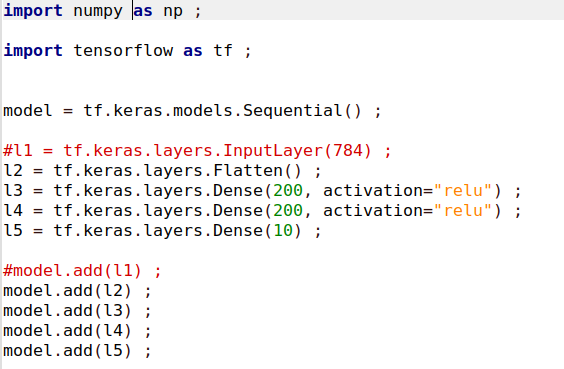
\includegraphics[width=0.5\textwidth]{snippet.png}
    \caption{Normalerweise bindet man Snippets als Bilder ein. Falls sie mehr als eine Viertelseite umfassen, bitte in den Anhang so wie hier gezeigt. Diese Snippets können dann trotzdem aus dem Text referenziert werden.\label{Snippet}
    }
\end{figure}
Binden Sie Snippets ein wie in \ref{Snippet} gezeigt!

\section {Generelle Hinweise}
\begin{itemize}
    \item Diese Vorlage ist nicht universell! Jede wissenschaftliche Arbeit ist anders. Daher: Halten Sie Kontakt zu Ihren Betreuer*innen und reden Sie mit ihnen über die konkrete Ausformung der Arbeit
    \item Sie müssen nicht LaTeX benutzen, Word ist auch ok. In jedem Fall muss die Form dieser Vorlage nachempfunden sein (Schriftgröße, Zeilenabstand, ...).
    \item Bei Fragen sind stets die Betreuer*innen die erste Anlaufstation, bitte nutzen Sie diese Möglichkeit, v.a. in den Sprechstunden!
    \item Generell wird das Gendern weder vorgeschrieben noch verboten, Sie können dies nach eigenem Ermessen gestalten. 
    \item Sprache: Deutsch oder Englisch
     \item Die Länge einer Arbeit kann variieren, je nach Thema. Bei Masterarbeiten sind ca. 50-55 Seiten der Median (ohne Anhänge), bei Bachelorarbeiten etwa 40-45.
     \item Besonderes Augenmerk sollte auf jeden Fall auf einer ansprechenden Form liegen (schöne und ausreichend viele Grafiken wo nötig, Formatierung, etc.) sowie der Sprache (keine Umgangssprache, elegantes Formulieren, Benutzung von Nebensätzen, ...) liegen, da diese beiden Punkte stark in die Note eingehen. Ebenfalls sehr wichtig (für die Benotung, aber auch so) sind die Kapitel Einleitung, Diskussion und Schluss, da oft nur diese gelesen werden. KI-Tools wie Grammarly können benutzt werden um die Sprache zu verbessern, ebenso wie Rechtschreib- und Grammatik-Checker (z.B. aspell). 
     \item Achten Sie bei Grafiken darauf, dass sie a) lesbar sind wenn das Dokument in A4-Größe betrachtet wird b) nicht verpixelt sind.
     \item Die Ich-Form ist zu vermeiden. Also 'es wurde festgestellt...' statt 'ich habe herausgefunden...'. Generell keine Prosa und chronologische Darstellung ('zuerst wurde das gemacht, dann das und dann das') sondern inhaltliche Gliederung!
     \item Abkürzungen, sofern sie nicht absolut offensichtlich sind, sollten bei der ertsen Benutzung eingeführt werden. Ein Abkürzungsverzeichnis kann sinnvoll sein, vor der Einleitung.
     \item Achten Sie darauf, Abschnitte nicht zu sehr zu verschachteln. Maximal zwei Unterebenen ist eine gute Regel (also 1.1.1 aber nicht 1.1.1.2). 
\end{itemize}
\section{Mehr zu Zitaten und Verweisen}
Zentral für das wissenschaftliche Arbeiten ist, dass man den Ursprung jeder Darstellung, sei es nun
eine Tatsache oder eine Bewertung, eindeutig kenntlich macht: \cite{shiny1}. Diese
Forderung hat drei Gründe:
\begin{itemize}
\item Man darf sich nicht „mit fremden Federn schmücken“, d.h. fremde Gedanken als die
eigenen ausgeben. Dies wäre der Fall, wenn man übernommene bzw. referierte Aussage
nicht als solche kenntlich macht.
\item  Man kann so die Lesenden auf weitere Literatur zur Vertiefung verweisen, wenn man aus
Platz- und Strukturgründen nicht selbst alle Details eines Gedankens oder Wissensbau-
steins referieren möchte. Dadurch kann man sich auf das Wesentliche beschränken,
welches zum Verständnis und wissenschaftlichen Einordnen der eigenen Arbeit wichtig ist.
\item Durch den genauen Nachweis oder Beleg wird sichergestellt, dass sich keine Fehler in
Form von falschen Zitaten in der Wissenschaft festsetzen können. Jeder kann durch den
Beleg genau die referierte Stelle im Original nachlesen und feststellen, ob der Autor richtig
verstanden und wiedergegeben wurde.
\item Man schützt sich durch das Belegverfahren davor, für fremde Fehler „gerade stehen zu
müssen“. D.h. wenn einem Autor ein Fehler unterläuft, den Sie in Ihrer Bachelor-
/Masterarbeit ohne Beleg wiedergeben, gilt das so, als ob Sie selbst diesen Fehler
gemacht haben. Wenn Sie aber belegen, wo Sie eine falsche Aussage, die Sie nicht als
falsch erkannt haben, „abgeschrieben“ haben, dann liegt die Verantwortung für den Inhalt
nicht bei Ihnen, sondern bei Ihrer Quelle.
\end{itemize}
Man unterscheidet zwischen zwei Arten von wissenschaftlichen Belegen, dem Verweis und dem
Zitat.
\subsection{Verweis}
Ein Verweis bezeichnet die sinngemäße Wiedergabe eines Sachverhalts in eigenen Worten. Nach
den entsprechenden Ausführungen wird der Verweis \cite{clemen1989combining} eingefügt. 
Eine gute Möglichkeit kenntlich zu machen, dass man sich auf einen bestimmten Autor bezieht, ist
die Verwendung solcher Formulierungen wie 'nach Darstellung in \cite{clemen1989combining} ...' oder 'Wie in \cite{clemen1989combining} ausgeführt, ...'.
\subsection{Zitat}
Ein Zitat bezeichnet die exakte wörtliche Wiedergabe aus einem Text. Ein Zitat muss immer in
Anführungszeichen stehen und mit Angabe der Quelle (genauso wie beim Verweis). Dies ist in der Informatik eher unüblich und sollte sehr sparsam eingesetzt werden.

\section{Hinweise zum Kolloquium}
Das Kolloquium besteht aus 15 Minuten Präsentation gefolgt von ca 20 Minuten Fragen zur Arbeit und Diskussion. Anwesend sind mindestens die beiden Gutachter, Dritte können ohne weitere Anmeldung ebenfalls dabei sein (Kolloquien sind öffentlich). 

Zielgruppe sollen Laien (z.B. höheres Management) sein, nicht die beiden Gutachter. Das bedeutet dass mindestens ein Drittel der Präsentation aus Motivation und Kontext besteht. Hier kann sich stark an die Einleitung der Arbeit angelehnt werden. Viele Bilder helfen ebenfalls, können aus der Arbeit sein.

Maximal soll die Präsentation 15 Slides enthalten (also maximal 1 Slide pro Minute). Es können zusätzliche Slides mit Details erstellt werden die vermutlich in der Diskussion sowieso gefragt werden.

Das Kolloquium ist nicht benotet, dh. es gibt nur bestanden oder nicht bestanden als Ergebnis. 

Generell sind die Studierenden verantwortlich für die Terminfindung und sollen nach Einreichung der Arbeit selbst aktiv werden. 

Tipps:
\begin{itemize}
    \item langsam sprechen! Laut sprechen!
    \item Unter Zeitdruck lieber ganze Folien weglassen als schneller sprechen
    \item Folien nummerieren
    \item Bitte unbedingt 15min vor dem Termin Hardware (Beamer, Headset, Kamera) testen. Das macht einen extrem schlechten Eindruck wenn dadurch Verzögerung entsteht
    \item niemals nur den Text der Folien vorlesen. Folien sollen sehr wenig Text und viele Bilder haben. Text soll nur Stichpunkte angeben, der Rest wird frei formuliert
    \item Kolloquien können ohne Weiteres online stattfinden!
    \item bei physischen Terminen: immer einen USB-Stick mit der Präsentation als PDF dabeihaben falls man einen anderen PC nutzen muss. PDF geht überall, PowerPoint nicht (und sieht v.a. nicht überall gleich aus)
    \item Totales No-Go: Rechtschreibfehler auf Folien
    \item Vermeiden Sie aufwändige Animationen oder Videos wenn möglich, kann immer sein dass das nicht funktioniert
\end{itemize}

%%%%%%%%%%%%%%%%%%%%%%%%%%%%
%% Eidesstattliche Erklärung
%% muss angepasst werden
%% in Erklaerung.tex
%%%%%%%%%%%%%%%%%%%%%%%%%%%%
\newpage
\begin{otherlanguage}{ngerman}
\thispagestyle{empty}
\section*{Eidesstattliche Erklärung}
\thispagestyle{empty}
Hiermit versichere ich, die vorliegende Arbeit selbstständig verfasst und keine anderen als die angegebenen Quellen und Hilfsmittel benutzt sowie die Zitate deutlich kenntlich gemacht zu haben.
\newline
Ich erkläre weiterhin, dass die vorliegende Arbeit in gleicher oder ähnlicher Form noch nicht im Rahmen eines
anderen Prüfungsverfahrens eingereicht wurde.
\vspace{4\baselineskip}\\
Würzburg, den \today \hfill Autor
\vspace{4\baselineskip}\\
\end{otherlanguage}

\end{document}
